\documentclass{article}
\usepackage[utf8]{inputenc}
\usepackage[margin=0.75in]{geometry}
\usepackage{enumerate}
\usepackage{amsmath}
\usepackage{amsfonts} 
\usepackage{amssymb}
\usepackage{amsthm}
\usepackage{mathtools}
\usepackage{float}
\usepackage{array}
\usepackage{makecell}
\usepackage{commath}
\usepackage{verbatim}

\DeclarePairedDelimiter{\ceil}{\lceil}{\rceil}

\renewcommand\theadalign{bc}
\renewcommand\theadfont{\bfseries}
\renewcommand\theadgape{\Gape[4pt]}
\renewcommand\cellgape{\Gape[4pt]}

\newcommand{\N}{\mathbb{N}}
\newcommand{\Z}{\mathbb{Z}}
\newcommand{\Q}{\mathbb{Q}}
\newcommand{\C}{\mathbb{C}}
\newcommand{\R}{\mathbb{R}}
\newcommand{\F}{\mathbb{F}}
\newtheorem{theorem}{Theorem}
\newtheorem{corollary}{Corollary}[theorem]
\newtheorem{definition}{Definition}[theorem]
\newtheorem{lemma}[theorem]{Lemma}
\newtheorem*{remark}{Remark}
\newcommand{\cdotscalar}{\;\widetilde{\cdot}\;}
\newcommand{\vectorplus}{\;\widetilde{+}\;}
\newcommand{\Span}{\text{Span}}
\newcommand{\Null}{\text{Null}}
\newcommand{\Range}{\text{Range}}
\newcommand{\D}{\frac{d}{\dif x}}

\renewcommand{\epsilon}{\varepsilon}
\renewcommand{\phi}{\varphi}

\newcommand{\Or}{\mbox{ OR }}
\renewcommand{\And}{\mbox{ AND }}
\newcommand{\Not}{\mbox{NOT }}
\newcommand{\Iff}{\mbox{ IFF }}

\newcommand{\Width}{\textup{width}}
\newcommand{\Mesh}{\textup{mesh}}
\newcommand{\Int}{\textup{Int}}
\newcommand{\Ext}{\textup{Ext}}
\newcommand{\Bd}{\textup{Bd}}


\newcommand\widebar[1]{\mathop{\overline{#1}}}
\newcommand*\closure[1]{\widebar{#1}}

\newcommand\Ball[2]{U(#1; #2)}

\begin{document}

\section*{Question 2: Feature Maps}

\begin{enumerate}[(a)]
    \item This data is not seperable by a linear classifier. We know that a linear classifier separating this data must partition $\R^2$ into half-spaces $H_1$ (positive) and $H_0$ (negative) based on a threshold $t$. 
    
    In this dataset, $p_1 = (-2, -1)$ and $p_2 = (2, 3)$ have label $1$, and so are in $H_1$. We know that half-spaces are convex, and so any convex combination of $p_1$ and $p_2$ must lie in $H_1$. If we take $\lambda = 3/4$, then 

    \[p_2 = p_1 + \lambda(p_2 - p_1) = (-2, -1) + \frac{3}{4}(2 - (-2), 3 - (-1)) = (-2, -1) + \frac{3}{4}(4, 4) = (1, 2)\]

    must lie in $H_1$ since it is convex combination of $p_1$ and $p_2$. However, we know that $p_3$ has label $0$, and so must lie in $H_0$. This is a contradiction, and so no linear classifier can separate this data.
    \item We will assume that a threshold $t = 0$ is used. The constraints are as follows:
    
    \begin{align}
        -2w_1 + w_2 &\geq 0\\
        w_1 + 4 w_2 &< 0\\
        2w_1 + 9w_2 &\geq 0
    \end{align}
    \item The feasible area is given by the intersection of the blue, red, and green half-spaces below, which is the shaded region to the left of the red line, above the green line, and below the blue line. The feasible area is shown in Figure \ref{fig:q2c}.
    
    \begin{figure}[H]
        \centering
        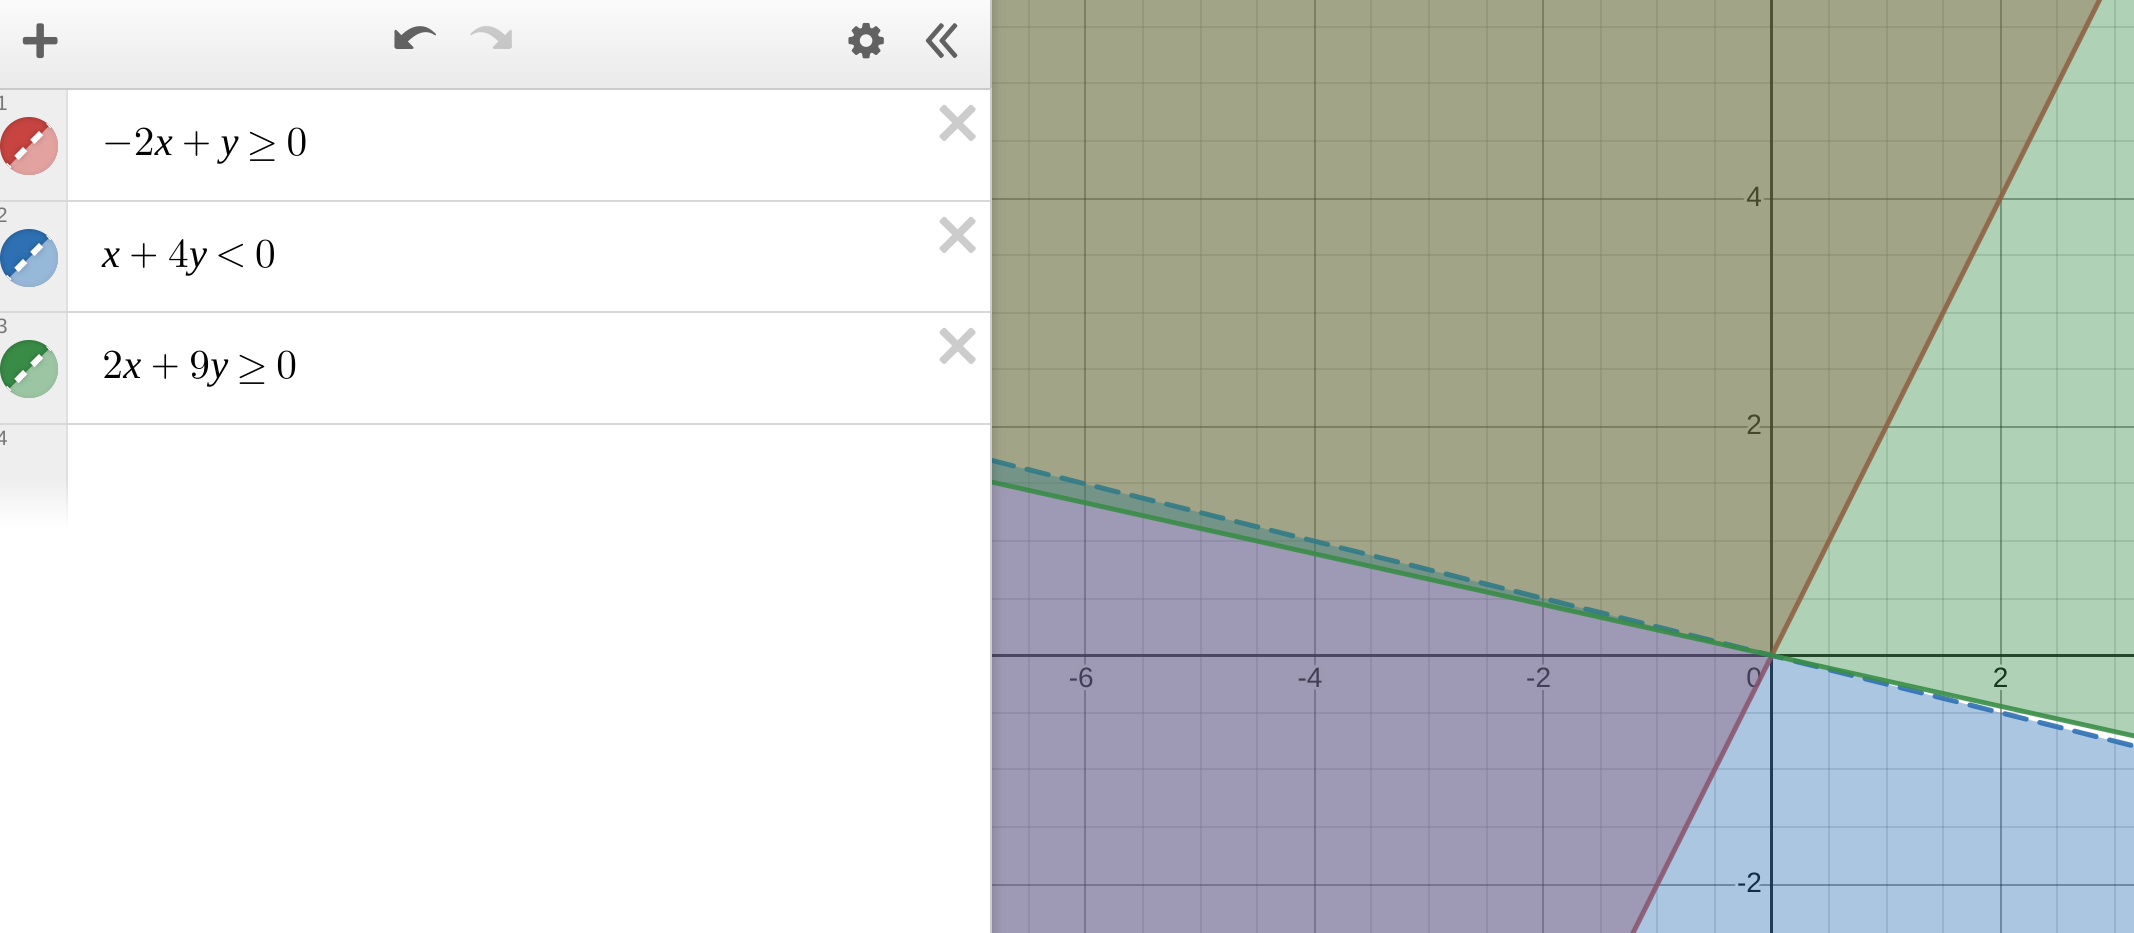
\includegraphics[width=0.9\textwidth]{../figures/q2_c_feasible_area.png}
        \caption{Feasible area for $w_1, w_2$}
        \label{fig:q2c}
    \end{figure}
\end{enumerate}

\newpage
\section*{Question 3: kNN vs Logistic Regression}

\begin{enumerate}[3.1]
    \item \begin{enumerate}[(a)]
        \item The plot of classification vs validation accuracy is given below in Figure \ref{fig:q3a}.
        
        \begin{figure}[H]
            \centering
            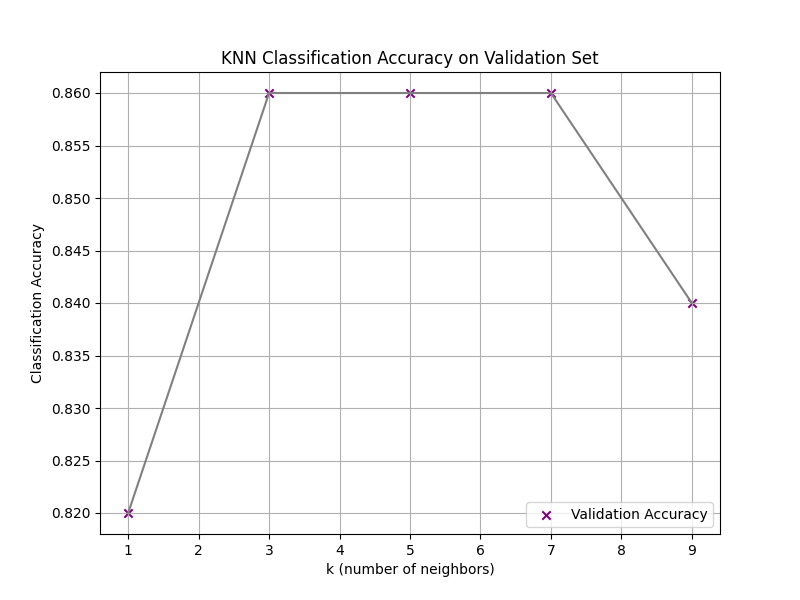
\includegraphics[width=0.7\textwidth]{../figures/knn_classification_accuracy.png}
            \caption{Classification vs Validation Accuracy}
            \label{fig:q3a}
        \end{figure}
    
        \item The value of $k^*$ chosen is $k^* = 3$. This is because $3$ is the smallest value of the hyperparameter $k$ which achieves the maximum accuracy seen across all values of $k$ (0.860). I have chosen this value of $k$ in adherence with the principle of Occam's Razor, which states that the simplest solution is often the best one. In this case, the simplest solution is the least complex model (lowest $k$), as the model complexity increases with $k$. 
        
        Here is a report of the validation and test accuracies for $k^*, k^* + 2, k^* - 2$:
    
        \begin{verbatim}
            Classification accuracies for k_star=3
                Validation accuracy: 0.86
                Test accuracy: 0.92
            Classification accuracies for (k    _star + 2)=5
                Validation accuracy: 0.86
                Test accuracy: 0.94
            Classification accuracies for (k_star - 2)=1
                Validation accuracy: 0.82
                Test accuracy: 0.88
        \end{verbatim}
    
        We see that the maximum validation accuracy is reached when $k^* = 3$, increasing from 0.82 when $k = 1$ and staying at the same value of 0.86 when $k = 5$.
        
        However, the test accuracy increases from $0.88$ to $0.92$ when going from $k^* - 2$ to $k^*$, and continues to increase with $k = k^* + 2 = 5$. This illustrates that the simplest model that performs best on the validation set may not always be the one that performs best on the test set. 
    \end{enumerate}
    
    \item \begin{enumerate}[(a)]
        \item Done!
        \item I've completed the missing parts in \texttt{run\_logistic\_regression}, and run the code on both \texttt{mnist\_train} and \texttt{mnist\_train\_small}. The value returned by \texttt{run\_check\_grad} is small, and is given below:
        
        \begin{verbatim}
            diff = 2.246931370781212e-08
        \end{verbatim}

        I used an initial value of $w = \vec{0}$, and a learning rate of $\eta = 0.2$. I chose this value as it was the largest value of $\eta$ that did not cause the loss to fluctuate in the early training iterations on both the training and validation sets.

        I used $500$ iterations, as it appears that both the cross entropy and classification accuracies converge on the training and validation sets after $500$ iterations.

        The cross entropy and classification accuracies for the training and validation sets for $\eta = 0.2$ and $500$ iterations are given below:

        \begin{verbatim}
            Classification accuracy on training set: 1.0
            Classification accuracy on validation set: 0.88
            Classification accuracy on test set: 0.92
            Cross entropy on training set: 0.02149375612870086
            Cross entropy on validation set: 0.19186085743772488
            Cross entropy on test set: 0.2142534589131518
        \end{verbatim}

        \item Here are figures showing how cross-entropy changes as training progresses, one for the \texttt{mnist\_train} and one for the \texttt{mnist\_train\_small} datasets.
        
        \begin{figure}[H]
            \centering
            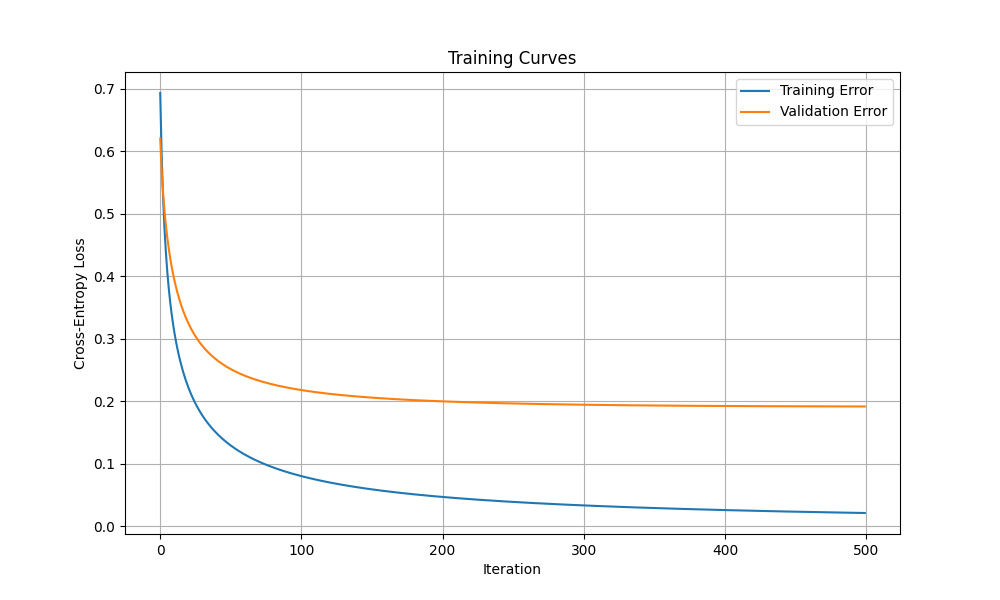
\includegraphics[width=0.7\textwidth]{../figures/mnist_train.png}
            \caption{Cross entropy vs Training Iterations for \texttt{mnist\_train}}
            \label{fig:q3b_mnist_train_cross_entropy}
        \end{figure}

        \begin{figure}[H]
            \centering
            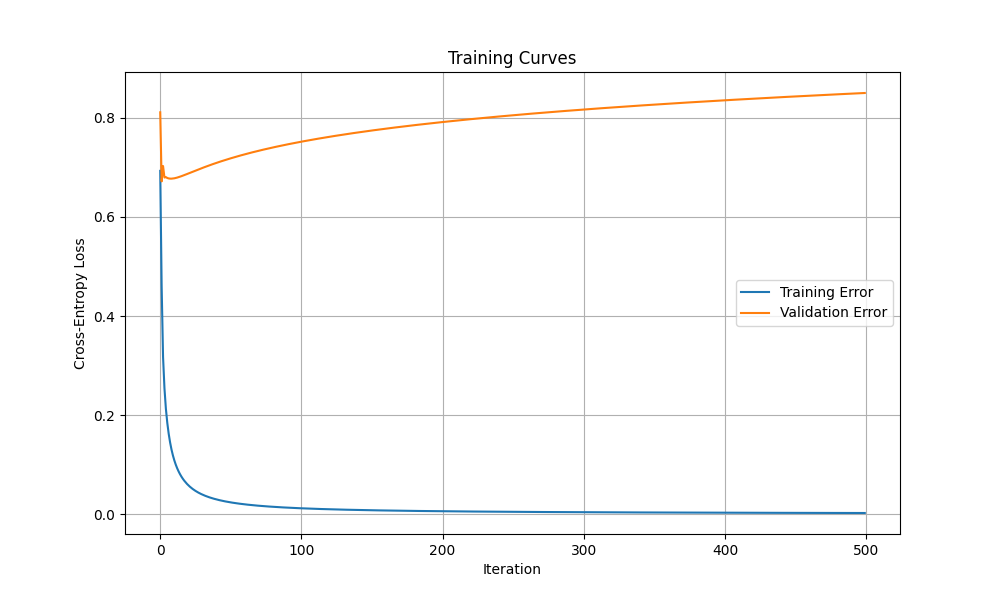
\includegraphics[width=0.7\textwidth]{../figures/mnist_train_small.png}
            \caption{Cross entropy vs Training Iterations for \texttt{mnist\_train\_small}}
            \label{fig:q3b_mnist_train_small_cross_entropy}
        \end{figure}

        We see that the validation error increases as the model trains on \texttt{mnist\_train\_small}, indicating that overfitting is taken place. No such phenomena is observed for \texttt{mnist\_train}, indicating that the model is not overfitting on this dataset.

        The results change with varying hyperparameters. Some ways to choose the best parame

    \end{enumerate}
\end{enumerate}
\end{document}